\section{$k$-a$n$o$n$: Secure Similarity Search in Outsourced Databases \cite{k-anon}}

	\begin{frame}[label={frame:knn}]

		\frametitle{General idea}

		\begin{itemize}
			\item<1->
				Model: \alert{snapshot}, query type: \alert{\knn{}} in arbitrary dimensions

			\item<2->
				Nearest-neighbor search needs definitions of \emph{object} and \emph{distance} \\
				\begin{small}
					\indent{} Object could be 2D/3D location, or a document embedding (high-dimensional vector) \\
					\indent{} Distance can be $\text{L}_\text{p}$ (usually, Euclidean, $p = 2$) or inner (dot) product
				\end{small}

			\item<3->
				Applications range from similarity search to geographical search \\
				\begin{small}
					\indent{} Object on a map is a 2D vector, query is to find $k$ nearest locations \\
					\indent{} Document is a vector of words/features/topics, query is to find $k$ most similar documents
				\end{small}

			\item<4->
				Our approach is to apply an \emph{approximate property-preserving encryption} on objects \\
				\begin{small}
					\indent{} Query protocol is then similar to OPE / ORE \\
					\indent{} Existing nearest-neighbor search algorithms then work naturally
				\end{small}

			\item<5->
				\textbf{Study how accuracy of search and efficiency of attacks drop with higher security}

		\end{itemize}

	\end{frame}

	\begin{frame}[label={frame:dcpe}]

		\frametitle{Distance Comparison Preserving Encryption}

		\[
			\forall x, y, z \in \mathbb{X} : \algo{Dist}{x, y} < \algo{Dist}{x, z} - \beta \implies \algo{Dist}{f(x), f(y)} < \algo{Dist}{f(x), f(z)}
		\]

		\begin{figure}[h]
			\centering
			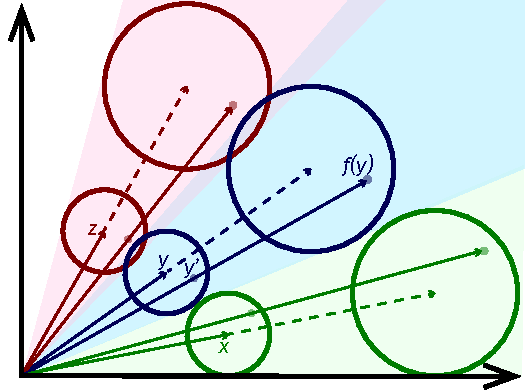
\includegraphics[width=0.5\columnwidth]{dcpe}
			\caption{
				Distance Comparison Preserving Encryption scheme \cite{dcpe} \\
				\hyperlink{frame:appendix:dcpe}{\beamerskipbutton{DCPE algorithms}}
			}%
		\end{figure}

	\end{frame}

	\begin{frame}{Search accuracy and TREC dataset}

		\begin{itemize}
			\item<1->
				Setup and query protocols: for given $\beta$
				\begin{itemize}
					\item Generate encryption key
					\item Encrypt dataset and queries set with $\beta$
					\item Run queries using conventional nearest-neighbor search (e.g., FAISS)
					\item Report search accuracy metrics
				\end{itemize}

			\item<2->
				TREC 2020 dataset is 8.8M documents embedded with fine-tuned BERT (768 dimensions) \\
				\begin{small}
					\indent{} Thanks Hamed Zamani for the dataset
				\end{small}

			\item<3->
				Query is a 768-dimensional embedding asking for $k = \num{1000}$ closest documents \\
				\begin{small}
					\indent{} TREC has a set of documents, a set of topics (questions), and relevance judgments (right answers)
				\end{small}

			\item<4->
				We report result set distance and difference, and ranking quality Recall, MRR and nDCG \\
				\begin{small}
					\indent{} Set distance and difference measure pure \knn{} accuracy \\
					\indent{} Recall, MRR and nDCG report ranking quality using relevance, common in information retrieval literature
				\end{small}

		\end{itemize}

	\end{frame}

	\begin{frame}{Search accuracy results}

		\begin{figure}[h]
			\centering
			\includegraphics[width=0.7\textwidth]{knn-search}
			\caption{Rank quality metrics, result set distance and difference for $\beta \in \{ 0, 1, \ldots , 50 \} $}
		\end{figure}

	\end{frame}

	\begin{frame}{Black-box inversion attack \cite{embedding-attacks}}

		\begin{itemize}
			\item<1->
				ML model trains on document-embedding pairs and predicts a \emph{set of words} from embedding \\
				\begin{small}
					\indent{} Model is an LSTM trained for 30 epochs \\
					\indent{} Original attack used BookCorpus \cite{bookcorpus} dataset, but we will use TREC
				\end{small}

			\item<2->
				We evaluate the attack on encrypted embeddings
				\begin{itemize}
					\item We also add plaintext and random embeddings for the baselines
					\item \textbf{Public model}: adversary can use \emph{the embedding model}, therefore, trains on plaintexts
					\item \textbf{Private model}: adversary can only use \emph{the entire system}, therefore, trains on ciphertexts
					\item In both cases the model predicts the words from the \emph{encrypted} embedding
				\end{itemize}

			\item<3->
				We measure precision, recall and \FOne{} score along with \emph{the percent of stop-words} \\
				\begin{small}
					\indent{} Stop-words are common words like ``a'', ``the'', articles, even punctuation and digits
				\end{small}

		\end{itemize}

	\end{frame}

	\begin{frame}{Attack performance results: public model (trained on plaintext)}

		\begin{figure}[h]
			\centering
			\includegraphics[width=0.8\textwidth]{knn-public}
		\end{figure}

	\end{frame}

	\begin{frame}{Attack performance results: private model (trained on ciphertext)}

		\begin{table}[!ht]
			\begin{tabular*}{\linewidth}{ !{\extracolsep\fill} l c c >{\bfseries}c c } % chktex 26
				\toprule
					Dataset							& Precision		& Recall	& \FOne{} score & \% of non-stop-words	\\
				\midrule
					Encrypted with $\beta = 0.0$	& 38.84			& 27.64		& 32.30			& 2.31					\\
					Encrypted with $\beta = 4.0$	& 36.28			& 26.61		& 30.70			& 3.21					\\
					Random embeddings				& 36.07			& 26.61		& 30.62			& 0.00					\\
				\bottomrule
			\end{tabular*}
		\end{table}

	\end{frame}

	\begin{frame}{Tradeoff between search accuracy and attack performance (public model, trained on plaintext)}

		\begin{figure}[h]
			\centering
			\includegraphics[width=0.8\textwidth]{knn-tradeoff}
		\end{figure}

	\end{frame}
